\chapter{Estudo de Casos}

\section{Primeiro Estudo de Caso}

A primeira etapa da arquitetura (coleta em campo) foi implementada em um notebook utilizando-se do SGBD (Sistema Gerenciador de Banco de Dados) PostgreSQL com a extensão espacial PostGIS, para dar suporte a dados convencionais e geográficos. Não importa qual a plataforma (linux ou windows) utilizada no notebook e nem a aplicação a ser desenvolvida (sistema de informação ou sistema de informação geográfico), o importante é ter um SGBD que funcione em várias plataformas e que suporte além dos dados convencionais, dados geográficos.
 
Já na segunda etapa da arquitetura, o módulo de captura de modificações foi desenvolvido com base na criação de \textit{triggers} que são disparadas quando ocorre uma operação de inserção, atualização ou deleção no banco de dados e armazena esses dados na tabela de auditoria com os seguintes dados adicionais: data e hora da operação (\textit{timestamp} da operação), usuário que realizou a operação, o \textit{host} de onde foi realizado a operação, o banco de dados onde ocorreu a ação, a tabela onde ocorreu a ação, a \textit{query} executada durante a ação, o valor antigo da tabela, o valor novo da tabela, uma \textit{flag} que indica se o registro já foi lido pelo módulo de transferência de modificações e etc \ref{fig:bdl} \ref{fig:auditoria}.

O módulo de transferência de modificações foi desenvolvido em java utilizando-se da biblioteca \textit{sync4j} do servidor \textit{Funambol Data Sync Server} (FUNAMBOL). Esse módulo nada mais é do que um cliente SyncML que consulta a tabela de auditoria, capturando as modificações no banco, e transfere as modificações ocorridas para o servidor de sincronização. O FUNAMBOL é um servidor de sincronização que implementa o protocolo SyncML e foi utilizado para implementar o servidor SyncML da arquitetura, com isso, todas as características do protocolo SyncML foram implementadas \cite{alonso}.

A última etapa, a etapa de armazenamento, foi desenvolvida através da replicação (\textit{backup}) dos dados do servidor de sincronização (FUNAMBOL) para o servidor de banco de dados, que foi desenvolvido com base no SGBD PostgreSQL com a extensão espacial PostGIS \ref{fig:servbd}.

Essa sincronização foi testada em diferentes tipos de redes (sem fio, com fio), em diferentes estados da rede (com pouca banda, com muita banda) e em diferentes níveis de segurança, e em todos os casos a sincronização foi bem sucedida. Tanto o módulo de captura de modificações como o módulo de transferência de modificações seguiram o diagrama apresentado no capítulo anterior, logo, possuem tolerância a falhas.

\begin{figure}[ht]
\centering
\includegraphics[width=250pt]{images/bdl.png}
\caption{Simulando uma inserção no banco de dados local, em um notebook.}
\label{fig:bdl}
\end{figure}

\begin{figure}[ht]
\centering
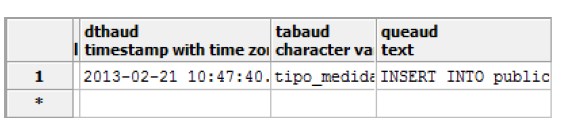
\includegraphics[width=250pt]{images/auditoria.png}
\caption{Tabela de auditoria.}
\label{fig:auditoria}
\end{figure}

\begin{figure}[ht]
\centering
\includegraphics[width=250pt]{images/servbd.png}
\caption{Servidor de banco de dados central.}
\label{fig:servbd}
\end{figure}
